\documentclass[11pt,a4paper,titlepage]{article}
\usepackage[utf8]{inputenc}
\usepackage[english]{babel}
\usepackage[T1]{fontenc}

\RequirePackage[layout=inline]{fixme}

\usepackage{float}
\usepackage{graphicx}
\usepackage{setspace}
\usepackage{amsmath}
\usepackage{courier}
\usepackage{amsmath}
\usepackage{listings}
\usepackage{color}
\usepackage[toc, page]{appendix}

\usepackage{algpseudocode}
\usepackage[bottom]{footmisc}
\usepackage{verbatimbox}

\usepackage{changepage}

\definecolor{mygreen}{rgb}{0,0.6,0}
\definecolor{mygray}{rgb}{0.5,0.5,0.5}
\definecolor{mymauve}{rgb}{0.58,0,0.82}




\lstset{ %
	backgroundcolor=\color{white},   % choose the background color
	basicstyle=\scriptsize,        % size of fonts used for the code
	breaklines=true,                 % automatic line breaking only at whitespace
	captionpos=b,                    % sets the caption-position to bottom
	commentstyle=\color{mygreen},    % comment style
	escapeinside={\%*}{*)},          % if you want to add LaTeX within your code
	keywordstyle=\color{blue},       % keyword style
	stringstyle=\color{mymauve},     % string literal style
	numbers=left,
}

%\renewcommand{\thesubsection}{\thesection.\alph{subsection}}



\usepackage{booktabs}
\usepackage[backend=biber, bibencoding=utf8, style=ieee]{biblatex}

\addbibresource{references.bib}
\usepackage[final,hidelinks]{hyperref} % must be last package loaded

\author{Ólafur Jón Thoroddsen}  % My name, for the titlepage
\title{\includegraphics{graphics/ru-logo}\\\vspace{10mm}
	Mechatronics II\\T-535-MECH \ \\Homework 7}  % The title, for the titlepage

\begin{document}
	\pagenumbering{arabic}
	\maketitle
	
	\tableofcontents
	\pagebreak
	
	\section{A Temperature Sensor For a Swimming Pool}
	
	Selecting a temperature sensor for a swimming pool must be done with care to ensure good measurements (see requirements) and minimize cost. I looked at three different sensors and compared their features to the list of requirements below.
	\subsection{Requirements\label{sec:requirements}}
	\begin{enumerate}
			\item\label{req:1}
			The sensor should be fairly accurate. We will accept a sensor which is accurate to at least $\pm 1^{\circ}\text{C}$.
			\item\label{req:2}
			The dynamic range of the sensor must be at least $0^{\circ}\text{C} - 50^{\circ}\text{C}$. It is very unlikely that the temperature will go outside that range.
			\item\label{req:3}
			Response time can be quite long, at least in the seconds timescale. The pool temperature might take minutes or tens of minutes to adjust to any changes. 
			\item\label{req:4}
			The sensor should be small so that it will not be a hindrance to anyone swimming in the pool.
			\item\label{req:5}
			It should be as inexpensive as possible.
			\item\label{req:6}
			The system should be easily scalable with more sensors.
	\end{enumerate}
	
	\subsection{National Semiconductors LM35\label{sec:lm35}}
	
	The LM35 temperature sensor is a very small and simple analog device that can be used with any microcontroller.
	
	\begin{table}[h]
		\centering
		\hspace*{-1cm}
		\begin{tabular}{llc}
			\toprule
			Req. num.	&	Attribute	&	\\
			\midrule
			1	&	Accuracy at $25^{\circ}\text{C}$	&	$\pm 0.5^{\circ}\text{C}$\\
			\midrule
			2	&	Dynamic range	&	$-55^{\circ}\text{C} - 150^{\circ}\text{C}$\\
			\midrule
			3	&	Time to reach final value (in stirred oil bath)	&	$\approx 3$ sec\\
			\midrule
			4	&	Physical dimensions (W$\times$H$\times$D)	&	4.7$\times$4.9$\times$4.2~mm\\
			\midrule
			5	&	Cost	&	\$1.5, approx. \$1.3 in bulk\\
			\midrule
			6	&	Scalability	&	\begin{tabular}{@{}l@{}}Requires an ADC\footnotemark. ATmega328p\\ can handle 6, for more, a \\dedicated ADC is needed\end{tabular}\\
			\bottomrule
		\end{tabular}
		\caption{LM35 attributes and features}
		\label{tab:lm35}
	\end{table}
	
	\noindent On paper, the LM35 looks pretty good. It has an unnecessarily wide dynamic range which could result in coarser data in our temperature range of interest then if the full dynamic range were utilized. It requires 3 wires, $\text{V}_{\text{cc}}$, GND and $\text{V}_{\text{out}}$.

	\footnotetext{Analog-Digital-Converter}
	
	
	\subsection{Maxim Integrated DS18B20}

	The DS18B20 is a more high end temperature sensor then the LM35. It is of a comparable size but it is a digital sensor rather then an analog one.

	
	\begin{table}[h]
		\centering
		\hspace*{-5mm}
		\begin{tabular}{llc}
			\toprule
			Req. num.	&	Attribute	&	\\
			\midrule
			1	&	Accuracy	&	$\pm 0.5^{\circ}\text{C}$ from $-10^{\circ}\text{C} - 85^{\circ}\text{C}$\\
			\midrule
			2	&	Dynamic range	&	$-55^{\circ}\text{C} - 125^{\circ}\text{C}$\\
			\midrule
			3	&	Response time	&	750ms in 12bit resolution mode\\
			\midrule
			4	&	Physical dimensions 	&	Not listed, about the same as LM35	\\
			\midrule
			5	&	Cost	&	\$4, approx. \$3.5 in bulk\\
			\midrule
			6	&	Scalability	&	\begin{tabular}{@{}l@{}}Each device has a unique 64bit\\address code, allowing multiple\\sensors to communicate on\\the same bus without hassle\end{tabular}\\
			\bottomrule
		\end{tabular}
		\caption{DS18B20 attributes and features}
		\label{tab:ds18b20}
	\end{table}
	
	With the DS18B20, it is easier to scale the system, allowing more sensors and thus increasing the accuracy of our pool temperature measurement. That would even allow for more sophisticated modeling and feedback control of the pool temperature. The sensor is quite expensive though, even when bought in bulk, approximately 3-4$\times$ as much as the LM35.
	There are 3 wires required, $\text{V}_{\text{cc}}$, GND and data (OneWire). The accuracy is rated very good for our entire working range.
	
	\subsection{Analog Devices TMP36}
	
	The TMP36 is a low cost temperature sensor that is included in hobby kits and supposedly indented for learning how to interface with analog sensors.
	
		\begin{table}[H]
			\centering
			\hspace*{-5mm}
			\begin{tabular}{llc}
				\toprule
				Req. num.	&	Attribute	&	\\
				\midrule
				1	&	Accuracy	&	$\pm 2^{\circ}\text{C}$ typical\\
				\midrule
				2	&	Dynamic range	&	$-40^{\circ}\text{C} - 125^{\circ}\text{C}$\\
				\midrule
				3	&	Response time	&	750ms in 12bit resolution mode\\
				\midrule
				4	&	Physical dimensions 	&	Not listed, about the same as LM35	\\
				\midrule
				5	&	Cost	&	\$4, approx. \$3.5 in bulk\\
				\midrule
				6	&	Scalability	&	\begin{tabular}{@{}l@{}}Each device has a unique 64bit\\address code, allowing multiple\\sensors to communicate on\\the same bus without hassle\end{tabular}\\
				\bottomrule
			\end{tabular}
			\caption{TMP36 attributes and features}
			\label{tab:tmp36}
		\end{table}
	
	The TMP36 is in the same price range as the LM35, has slightly narrower dynamic range (which is ok and might actually be good in this application). It's more inaccurate then both LM35 and DS18B20 with a 2-4$\times$ larger error margin.
	
	\subsection{Conclusion}
	
	For my pool project, I will go with the LM35 from National Semiconductors. It is less expensive then the DS18B20, relatively accurate for the required temperature range (good enough) and has actually better accuracy then the TMP36. It has a great response time, well within the required limits, and it is tiny, allowing it to be implemented in a multitude of situations.
	
	\begin{figure}[H]
		\centering
		\includegraphics[width=0.8\textwidth]{Arduino_LM35}
		\caption{Connection diagram for the LM35 to an Arduino}
	\end{figure}
	
	
	\subsection{Implementing the LM35 using the ATmega328p ADC}
	
	Because the LM35 is an analog temperature sensor, the voltage it produces must be converted to a digital value for the Arduino to interpret it.
	The ATmega328p has a 6 channel, 10bit ADC that is good enough for the pool project. It is initialized using the following registers: ADC Control and Status Register A (\verb|ADCSRA|) and ADC Multiplexer Selection Register (\verb|ADMUX|).
	
	\lstinputlisting[language=c,frame=single,firstline=10,lastline=16,firstnumber=10]{../adc_temp/adc.c}
	
	\noindent Line 11 sets the ADC clock at a 1/128th of the system clock, yielding a sampling rate of 125.000Hz. Setting the \verb|REFS0| bit in \verb|ADMUX| sets the analog reference voltage to $\text{V}_{\text{cc}}$. Setting \verb|ADATE| in \verb|ADCSRA| sets the ADC up in free-running mode, allowing continuous values to be read from the ADC Data Register (\verb|ADCL| and \verb|ADCH|). Lines 14 and 15 enable the ADC and start conversion respectively.
	
	Reading data from the ADC is implemented in a \verb|analogRead()| function as shown below.
	\lstinputlisting[language=c,frame=single,firstline=18,lastline=25,firstnumber=18]{../adc_temp/adc.c}
	
	\noindent Because the ADC is 10bit, it requires two 8bit registers to interface with (\verb|ADCl| and \verb|ADCH|). To capture all the data, we store it in a 16bit variable \verb|adc_val|, shifting the bits in \verb|ADCH| to the left by 8 positions and store the bits in \verb|ADCL| in the lower byte of \verb|adc_val|.
	
	\subsubsection{Testing the sensor}
	
	To test the program, a simple main.c file was created that calls the \verb|analogRead()| function on command. As as simple test, I held the LM35 tightly in my hand for a few seconds, measured the temperature and watched the terminal screen as it dropped towards room temperature.
	
	\lstinputlisting[language=c,firstline=15,lastline=28,frame=single,firstnumber=15]{../adc_temp/main.c}
	
	\begin{figure}[H]
		\centering
		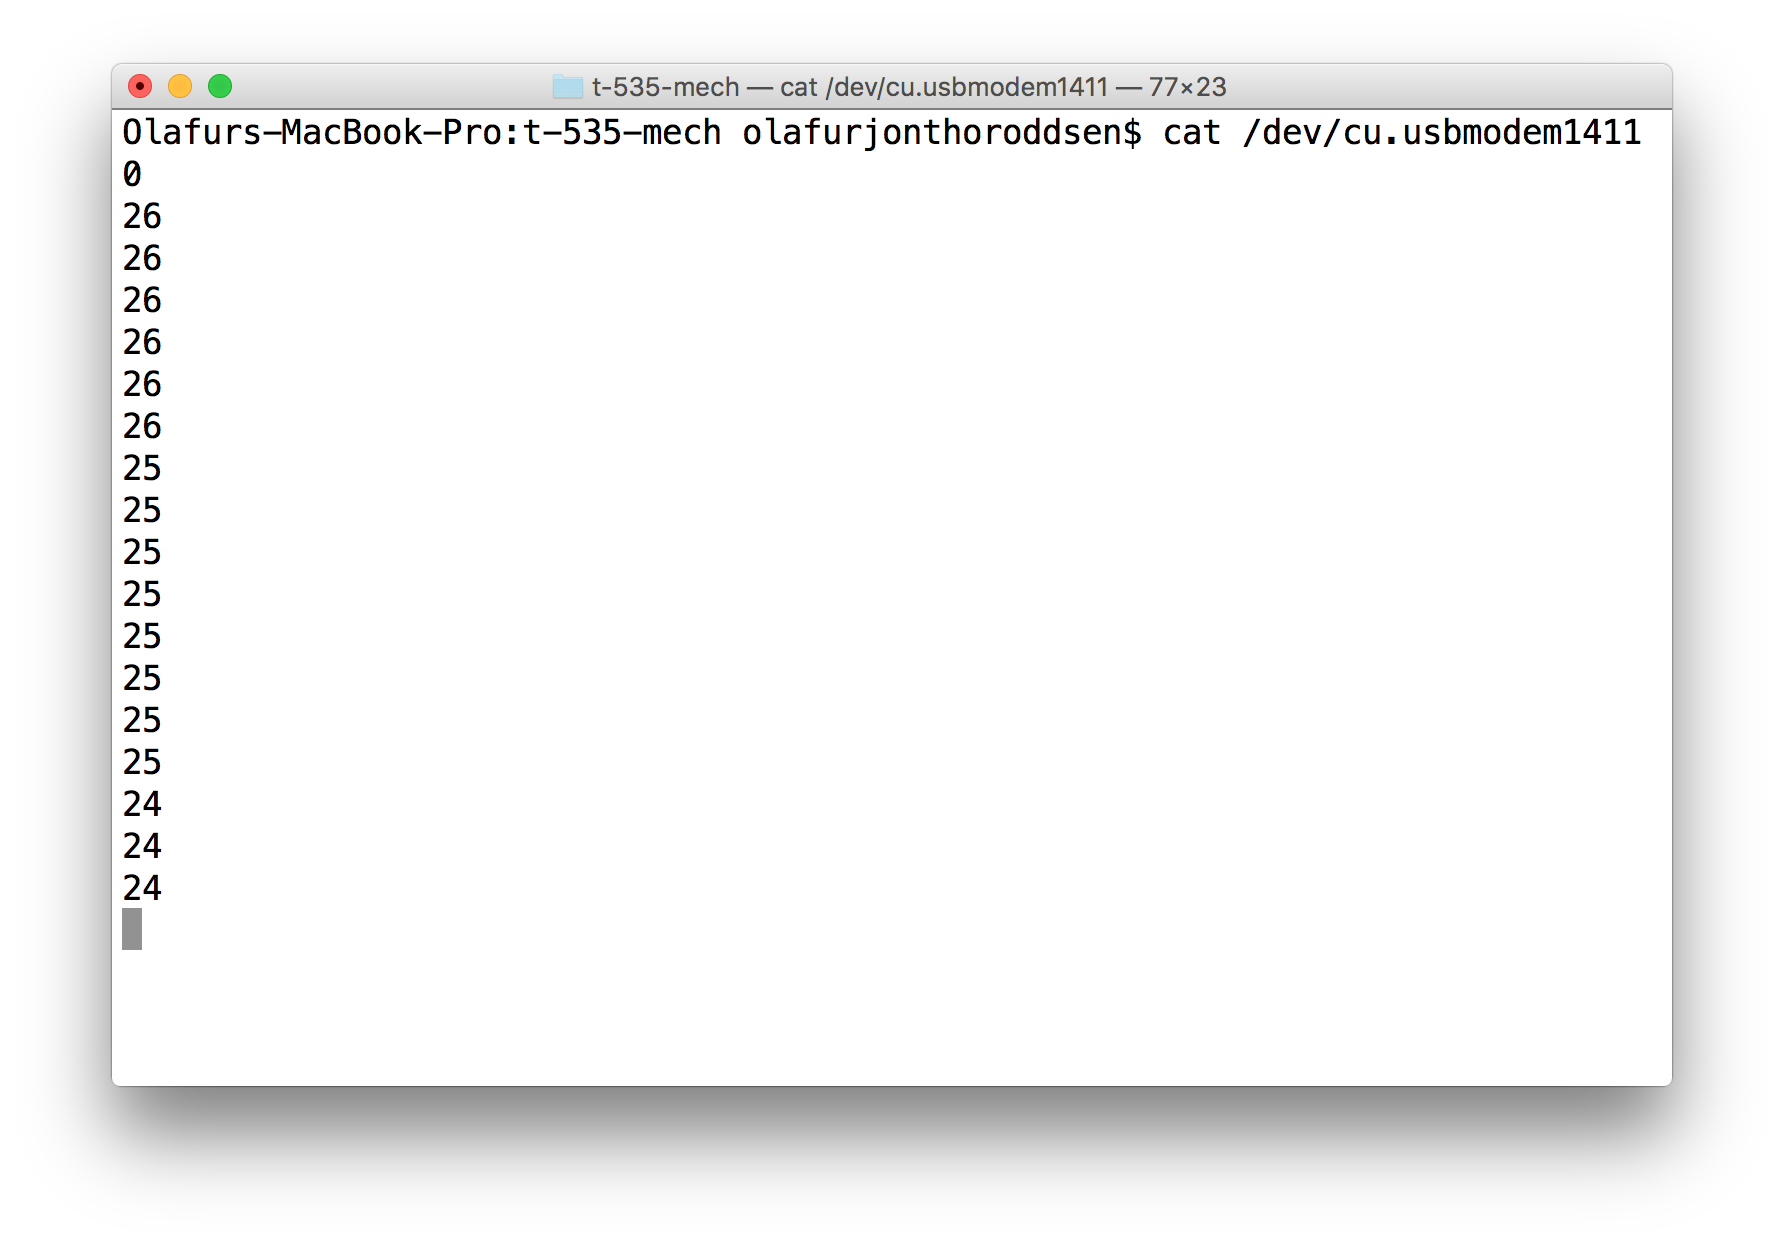
\includegraphics[width=\textwidth]{graphics/temp}
		\caption{Output from the temperature sensor after releasing it from my hand}
		\label{fig:temp}
	\end{figure}
	
	\pagebreak
	\section{Connecting a button}
	
	The schematic in figure~\ref{fig:button} shows how to connect a button to a digital pin on the Arduino.
	
	\begin{figure}[H]
			\centering
			\includegraphics[width=0.8\textwidth]{graphics/button}
			\caption{A schematic showing how to connect a button to an Arduino}
			\label{fig:button}
	\end{figure}
 	
 	\subsection{Software debouncing\label{sec:debounce}}
 	
 	Debouncing is a technique used to eliminate fluctuations in the input signal of a sensor or peripheral. I designed a software solution to this problem, utilizing the timers on board the ATmega328p.
 	
 	The basic strategy is to detect a change in the input pin and reset a timer once that happens. Then at specified intervals, we check if the pin status has changed, and if it has not changed between intervals and its value is HIGH, then we declare that the button was indeed pressed.
 	
 	There are some unnecessary variables in the code shown below because I intended to implement a more sophisticated finite state machine for counting the number of button pushes.
 	
 	\lstinputlisting[language=c,frame=single,firstline=9,firstnumber=9]{../button_debounce/main.c}
	
	\subsubsection{Testing the button}
		By hooking up a button like shown in figure~\ref{fig:button} and uploading the main.c program from~\ref{sec:debounce} onto the Arduino.
		The number of button pushes is kept track of in the terminal screen as seen in figure~\ref{fig:buttontest}.
		
		\begin{figure}[H]
			\centering
			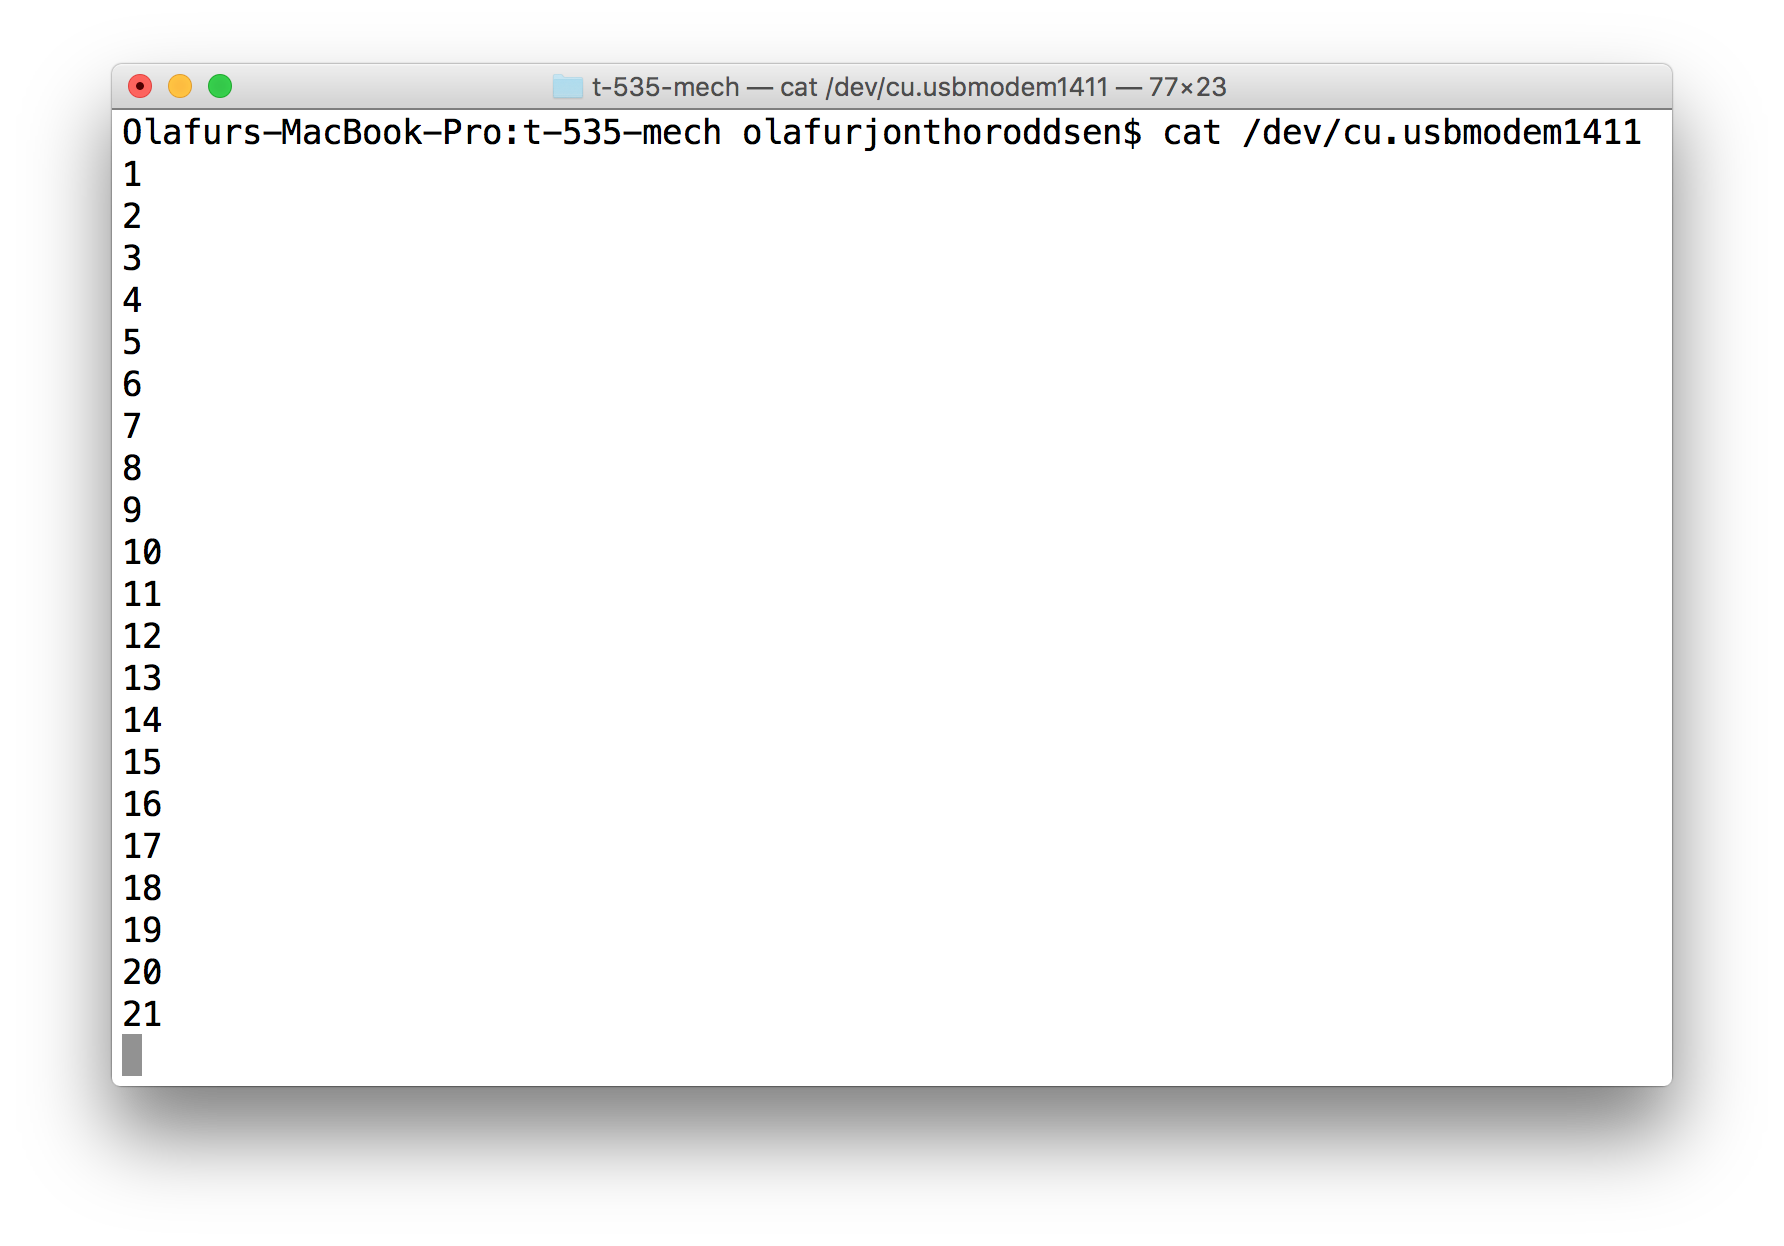
\includegraphics[width=\textwidth]{graphics/buttontest}
			\caption{The terminal readout from the button test.}
			\label{fig:buttontest}
		\end{figure}
	
	\pagebreak
	\section{Progress with my project}
	
	\subsection{Last week}
	This week I did not finish as much as I intended because of too much workload in other courses. I thought a lot about the dynamics of the robot and analyzed it more thoroughly then I had done before. I tried to contact Ármann about advice for the analysis but he did not respond to my email.
	
	As a result, next weeks plan is unchanged from last week and I will continue to work on sensor readout, PWM and planing the control system.
	
	\subsection{Next week}
	
	\begin{table}[h]
		\centering
		\begin{tabular}{llc}
			\toprule
			Task no.	&	Task	&	ETC\footnotemark\\
			\midrule
			1	&	\begin{tabular}{@{}l@{}}Debug the IMU sensor readout\\\end{tabular} &	5 hours \\	
			\midrule	
			2	&	\begin{tabular}{@{}l@{}}Find out if the PWM\\ functionalities in ATmega are\\worth replacing my own with.\end{tabular}	&	2 hours\\
			\midrule
			3	&	\begin{tabular}{@{}l@{}}If worth pursuing further, write a \\PWM module using the ATmega\\built in functionalities\end{tabular}	&	10 hours\\
			\midrule
			4	&	\begin{tabular}{@{}l@{}}Test the accuracy of the\\IMU sensor\end{tabular}	&	5 hours\\
			\midrule
			5	&		\begin{tabular}{@{}l@{}}Plan the control system and\\start designing at a high level\end{tabular}	&	5 hours\\
			\bottomrule
		\end{tabular}
		\label{tab:nextweek}
	\end{table}
	
	
	\footnotetext{Estimated Time to Complete}
	\pagebreak
	\subsection{Long term plan}
	
	\begin{table}[h]
		\centering
		\hspace*{-2cm}
		\begin{tabular}{lccc}
			\toprule
			Week	&	Software design	&	Mechanical design	&	Testing\\
			\midrule
			8	&	PID, PWM	&	Robot chassis	&	IMU \& PWM\\
			\midrule
			9	&	Rethink IMU \& PWM	&	\begin{tabular}{@{}l@{}}Power circuitry\\2nd prototype\end{tabular}	&	\begin{tabular}{@{}l@{}}Estimate power consumption\\PID motor control\end{tabular}\\
			\midrule
			10	&	Rethink PID control	&	3D drawing of the robot	&	Power consumption	\\
			\midrule
			11	&	\begin{tabular}{@{}l@{}}Integrate IMU, PID\\ and PWM modules\end{tabular}	&	Altium schematics of electronics	&	Integration\\
			\midrule
			12	&	Integration	&	Integration	&	Integration	\\
			\bottomrule
		\end{tabular}
		\label{tab:longterm}
		\hspace*{-2cm}
	\end{table}
	
	
\pagebreak
%\section*{Appendices}
\appendix



\pagebreak
\printbibliography

\end{document}